\newpage
\section{Experiments}~\label{experiment}
We first evaluate the task success rate of the proposed system and analyze the effect of query frequency. If a query is triggered, we assume that the human always provides the correct answer. Through preliminary experiments, we found that $\tau=0.8$ provides a reasonable trade-off between task performance and the number of queries. The success rates under different values of $\tau$ are reported in Appx.~\ref{appx:tau}. We then conduct a user study to evaluate how query frequency affects user workload. Finally, we conduct another user study using the same survey protocol to examine what to query. We compare our method with the KnowNo framework and analyze whether querying state-level information or action-level decisions results in lower user workload.

\begin{figure}[t!]
    %\captionsetup{skip=0pt} % \hspace{0.3cm}
    \begin{center}
  
    \begin{subfigure}[b]{0.47\textwidth}
        \captionsetup{skip=0pt}
	    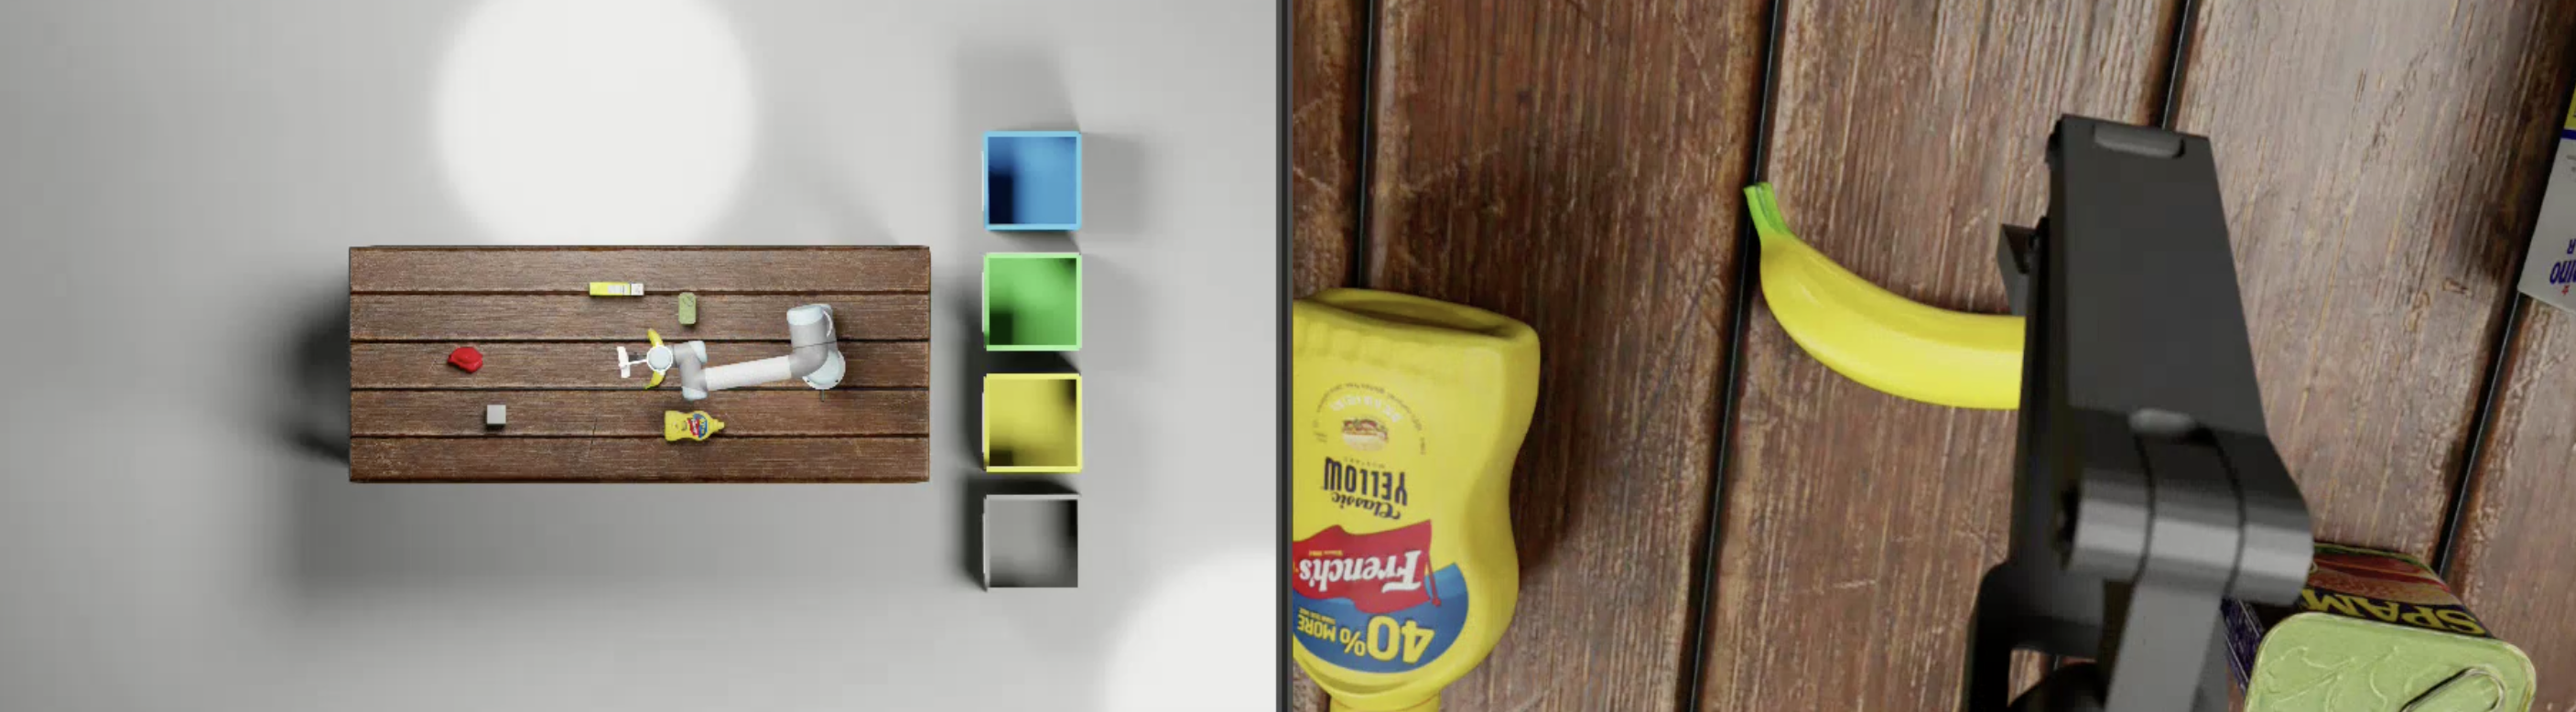
\includegraphics[width=\textwidth]{figures/fig_exp_setup1.png}
        \caption{Waste sorting domain overview. }
        \label{fig:dom1}
    \end{subfigure}
    \quad
    \begin{subfigure}[b]{0.47\textwidth}
        \captionsetup{skip=0pt}
	    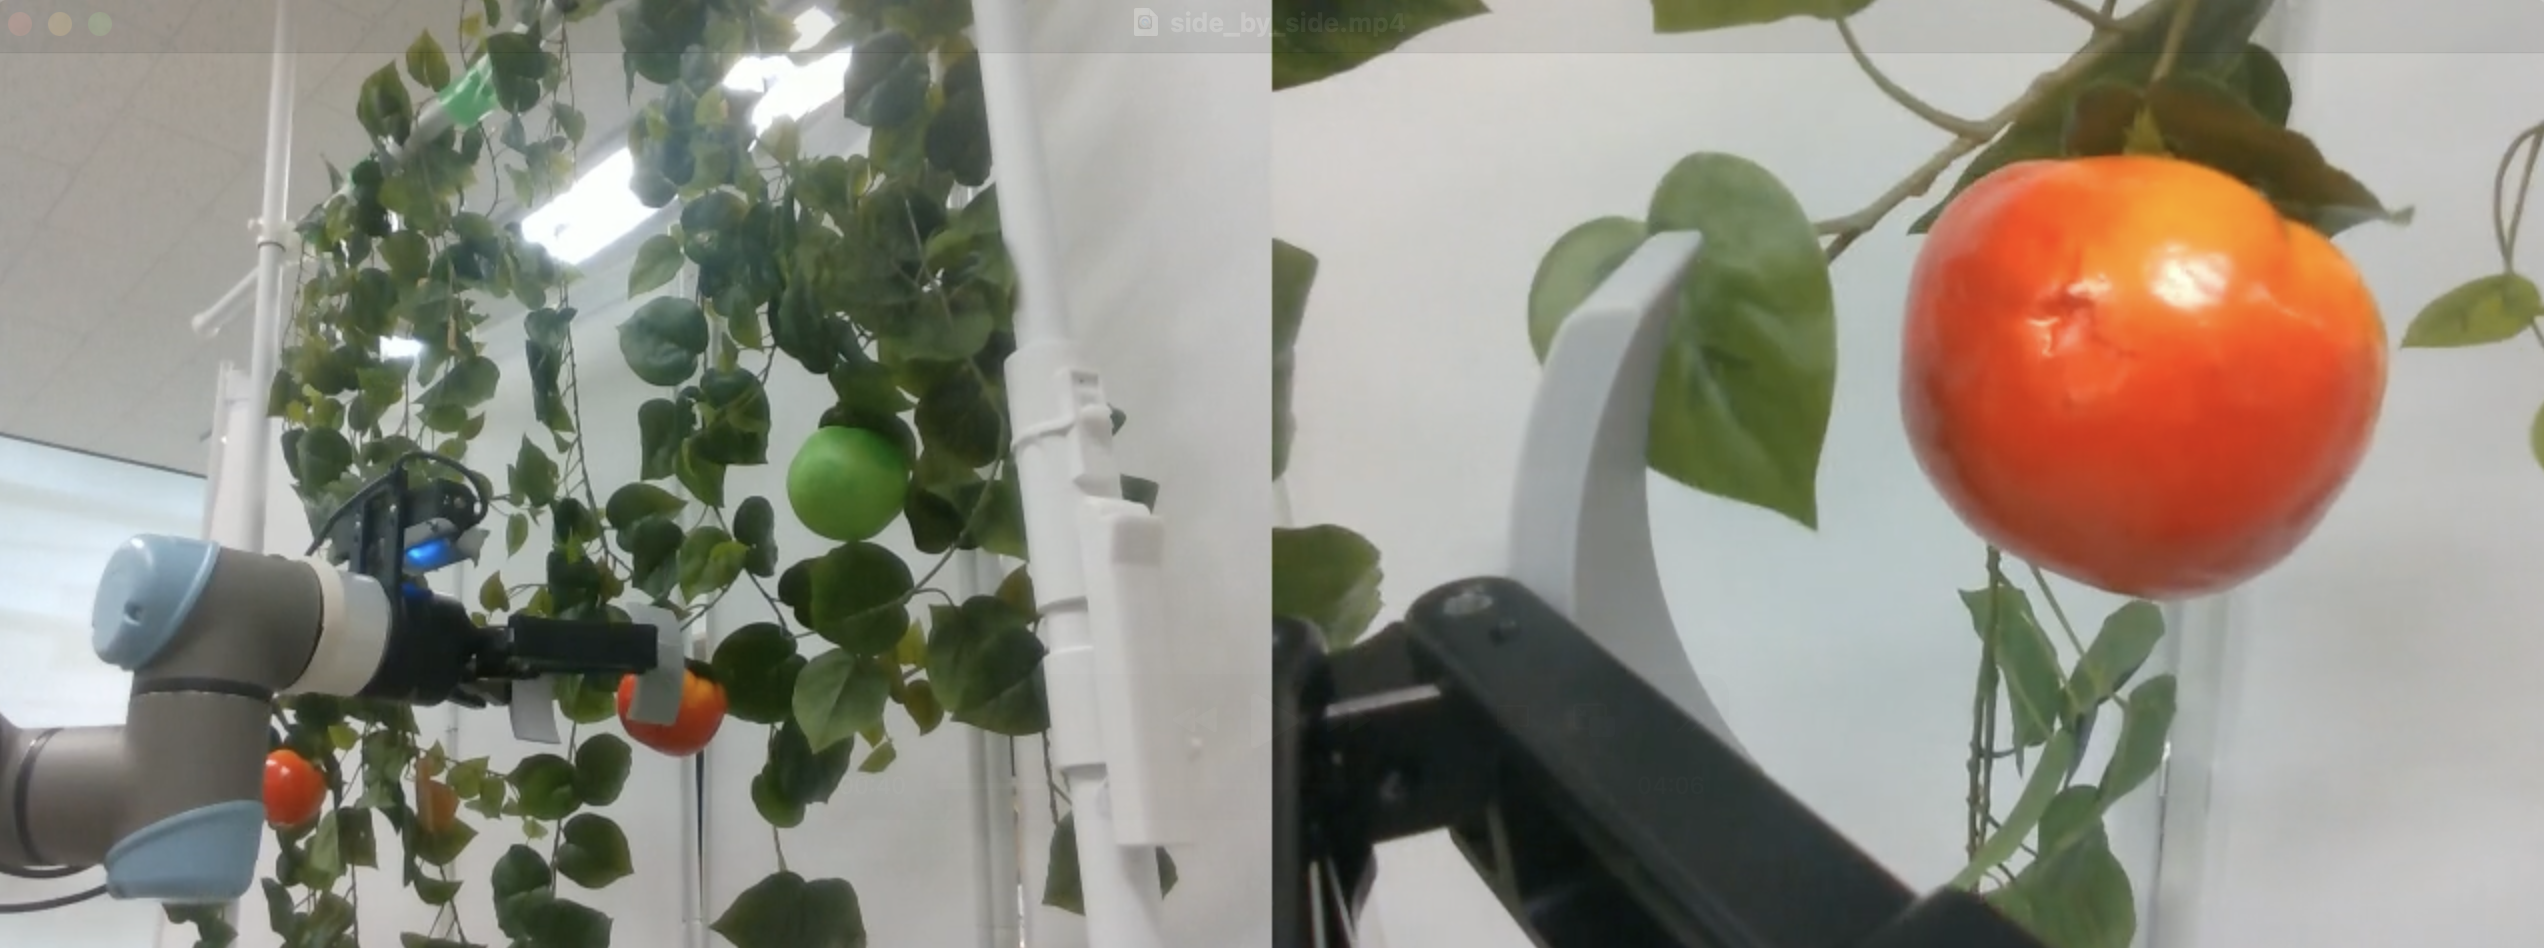
\includegraphics[width=\textwidth]{figures/fig_exp_setup2.png}
        \caption{Tomato harvesting domain overview}
        \label{fig:dom2}
    \end{subfigure}
    \caption{The illustration of the environments. (a) A UR5 robot sorts four types of waste into designated bins in Isaac Sim. (b) A mobile manipulator harvests ripe tomatoes and discards rotten ones in a real-world setting.}
  \label{fig:env_setting}
  
  \end{center}
\end{figure}


\subsection{Experimental Setup}~\label{exp:setup}
We evaluate the proposed method in two domains: a simulated waste sorting domain and a real-world tomato harvesting domain. The waste sorting domain is implemented in simulation using NVIDIA Isaac Sim, where a fixed UR5 robotic arm is used for pick and place task. Object detection is performed using the YOLOv12 model~\cite{tian2025yolov12}. In contrast, the tomato harvesting domain is deployed on a real mobile manipulator consisting of a UR5e robotic arm mounted on a Summit mobile platform. The robot is equipped with an RGB-D camera for visual perception and a LiDAR sensor for localization, and performs object detection using the same YOLOv12. 


\subsubsection{Waste sorting domain}~\label{exp:setup_waste}
We consider a tabletop waste-sorting scenario with four waste objects placed on a table, as shown in Fig.~\ref{fig:dom1}. A fixed UR5 robot is positioned between the objects and the recycling bins and performs three actions: \texttt{detect}, \texttt{pick}, and \texttt{place}. We assume that all objects are reachable by the manipulator.

Each object belongs to one of four categories: \texttt{general}, \texttt{paper}, \texttt{can}, and \texttt{plastic}. The object categories are not known a priori and must be inferred through perception. Since objects may be partially occluded by others, a single observation may not reveal all categories, requiring repeated detection during execution. The \texttt{detect} action can observe multiple objects simultaneously, after which the robot places each object into the corresponding recycling bin.

The initial arrangement of objects is randomized in every episode. A task is considered successful when all objects are correctly sorted within the maximum step limit. A reward of $+5$ is assigned when a waste object is placed into the recycling bin corresponding to its category, and an additional reward of $+10$ is given when all objects are correctly sorted. All other actions receive zero reward.



\subsubsection{Tomato harvesting domain}~\label{exp:setup_tomato}
We consider a tomato harvesting scenario in which four tomatoes are attached to two stems, denoted as \texttt{stem\_1} and \texttt{stem\_2}, as shown in Fig.~\ref{fig:dom2}. The robot navigates between three locations: \texttt{dock\_station}, \texttt{stem\_1}, and \texttt{stem\_2}, and performs \texttt{detect}, \texttt{pick}, \texttt{scan}, \texttt{place}, and \texttt{discard} actions.

Each tomato can be in one of three states: \texttt{ripe}, \texttt{unripe}, or \texttt{rotten}. The tomato states are initially unknown and must be estimated through perception. During detection, ripe and rotten tomatoes are visually ambiguous and cannot always be reliably distinguished. To resolve this ambiguity, the robot performs a \texttt{scan} action after picking a tomato to verify its condition before harvesting or discarding it. Unripe tomatoes are left untouched.

The tomato locations are randomized across stems in every episode. A task is considered successful when all ripe tomatoes are harvested and all rotten tomatoes are discarded within the maximum step limit. A reward of $+5$ is assigned when a ripe tomato is correctly harvested or a rotten tomato is correctly discarded after scanning. An additional reward of $+10$ is given when all task-relevant tomatoes are processed correctly. All other actions receive zero reward.



\subsubsection{Implementation Details}~\label{exp:details}
In all experiments, the planner used a discount factor $\gamma=0.95$, UCB exploration constant $c=1.0$, maximum simulation depth $depth_{\max}=20$, and $\Timeout=100$ Monte Carlo simulations per planning step. Each episode was limited to $50$ steps. The confidence threshold for triggering user feedback was set to $\tau=0.8$, which was selected empirically based on preliminary experiments (see Appx.~\ref{appx:tau}).

% \subsubsection{Evaluation Metrics}~\label{exp:metrics}
% \cp{We evaluate the proposed method based on task performance and human workload. Task performance is quantified using the task success rate, defined as the percentage of episodes in which the robot reaches the goal state required by each domain within maximum steps. An episode is considered a failure if the planner reaches a dead-end state or exceeds the maximum step limit. To assess the efficiency of human intervention, we additionally report the query frequency, measured as the average number of queries per episode. For the user studies, we employ the NASA-TLX questionnaire to evaluate subjective workload. Furthermore, we compare our state-level querying strategy with the KnowNo framework, which queries action-level decisions, to analyze their respective impacts on user workload and task success.}


\subsection{System Evaluation}~\label{exp:sys_eval}
We evaluate the proposed system in terms of task success rate and query efficiency under different querying strategies. In all experiments, if a query is triggered, we assume that the user always provides the correct answer in order to isolate the effect of the querying strategy itself. We compare four variants: \textbf{Ours}, \textbf{All}, \textbf{Random}, and \textbf{No}. The \textbf{Ours} method selectively queries the user if the confidence of the current belief falls below the threshold $\tau=0.8$. The \textbf{All} baseline requests user feedback at every decision step, corresponding to full human supervision. The \textbf{Random} baseline randomly triggers queries with the same average query frequency as \textbf{Ours}, without considering the belief confidence. The \textbf{No} baseline performs fully autonomous execution without any user feedback.

For each domain, we measure the task success rate, the average number of queries per episode, and the query ratio, which denotes the percentage of execution steps that triggered user feedback. In addition, we analyze how selective querying affects belief refinement during execution.


Table~\ref{tab:system_eval} summarizes the experimental results. In both domains, \textbf{All} achieves the highest task success rate because all ambiguities are resolved through continuous human supervision. In contrast, \textbf{No} shows a substantial decrease in performance due to accumulated perception errors and unresolved uncertainty during planning and execution.

The proposed method achieves a task success rate close to \textbf{All} while significantly reducing the number of queries. In the waste sorting domain, \textbf{Ours} achieves a success rate of XX.X\% while reducing the average number of queries from XX.X to XX.X. Similarly, in the tomato harvesting domain, \textbf{Ours} maintains comparable task performance while requiring substantially fewer user interactions. These results indicate that selective querying can effectively resolve critical uncertainty without relying on continuous user supervision.

In contrast, \textbf{Random} exhibits lower task success rates despite using a similar number of queries as \textbf{Ours}. This result suggests that the timing and content of queries are important, and that randomly requesting feedback does not reliably resolve task-relevant ambiguity.

The proposed system triggers queries only when the confidence of the current belief becomes sufficiently low. In practice, such situations occur when multiple candidate states explain the current observation with similar likelihoods. For example, in the tomato harvesting domain, ripe and rotten tomatoes may appear visually similar during distant observation, while in the waste sorting domain, partially occluded objects may lead to ambiguous category predictions.

When a query is triggered, the system selects the hypothesis expected to reduce the uncertainty the most and filters the belief based on the user response. As a result, the belief distribution becomes concentrated on a smaller set of candidate states, allowing the planner to continue execution with higher confidence. Across both domains, we observe that most task failures in the \textbf{No} baseline originate from unresolved ambiguity, whereas the proposed method successfully avoids many of these failures through selective user feedback.




Overall, the experimental results demonstrate that the proposed framework can maintain high task performance while substantially reducing the amount of required human feedback. Unlike the \textbf{All} baseline, the system does not rely on continuous supervision, and unlike \textbf{No}, it can recover from uncertain observations through interaction. These results suggest that confidence-based selective querying provides an effective balance between autonomy and human intervention in partially observable robotic tasks. 



\begin{table*}[t]~\label{{tab:system_eval}}
\centering
\caption{System evaluation under different querying strategies. \textbf{All} queries the user at every decision step, \textbf{No} performs fully autonomous execution without queries, and \textbf{Ours} selectively queries the user based on belief confidence ($\tau=0.8$). Query ratio denotes the percentage of execution steps that triggered user feedback.}
% \resizebox{\textwidth}{!}
\begin{tabular}{llcccc}
\toprule
\textbf{Domain} & \textbf{Method} & \textbf{Task Success Rate (\%)} & \textbf{Average Queries} & \textbf{Query Ratio (\%)} \\
\midrule

\multirow{3}{*}{Waste Sorting}
& \textbf{All}  & 98.0 & 12.4 $\pm$ 0.0 & 100.0 \\
& \textbf{No}   & 71.5 & 0.0 $\pm$ 0.0  & 0.0 \\
& \textbf{Ours} & 94.5 & 3.1 $\pm$ 1.4  & 25.0 \\
\midrule

\multirow{3}{*}{Tomato Harvesting}
& \textbf{All}  & 96.0 & 10.6 $\pm$ 0.0 & 100.0 \\
& \textbf{No}   & 68.0 & 0.0 $\pm$ 0.0  & 0.0 \\
& \textbf{Ours} & 92.5 & 2.8 $\pm$ 1.1  & 26.4 \\
\bottomrule
\end{tabular}
\end{table*}








\subsection{User Study}




\subsection{Discussion}